\chapter{}

\section{Enunciado}

Implementar un codificador y decodificador de mensajes haciendo uso de máquinas de Mealy.

\section{Solución}

Vamos a crear una máquina de Mealy que codifique un mensaje que trabaje con dos procesos de codificación:
Invertir ceros ($q_0$) y unos o reproducirlos sin inversión ($q_1$).
La máquina empezará codificando en el primer modo y, después de leer un \texttt{1} y codificarlo en el modo actual, cambiará de modo.

\begin{figure}[h!]
\begin{center}
	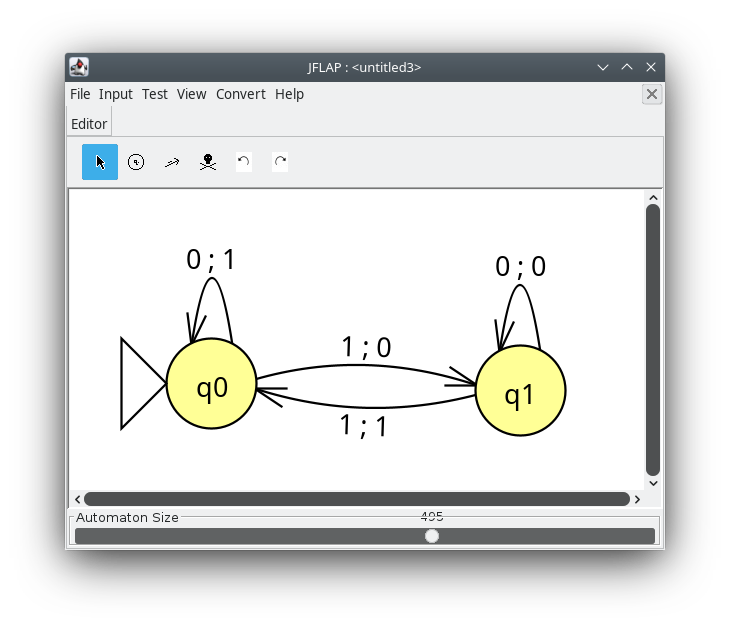
\includegraphics[scale=0.34]{Prácticas/Mealy - Codificador}
	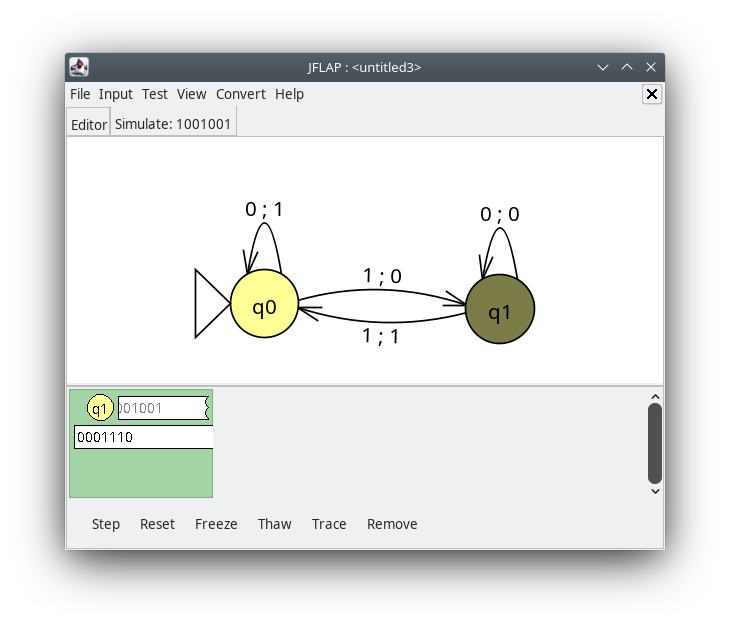
\includegraphics[scale=0.34]{Prácticas/Mealy - Codificador ejecución}
\end{center}
\caption{Máquina de Mealy codificadora.}
\end{figure}

Para crear un decodificador, hacemos lo mismo pero indicando que el cambio de modo se realice después de leer un \texttt{0}.
Lo probamos introduciendo la cadena resultante de la ejecución anterior.

\begin{figure}[h!]
\begin{center}
	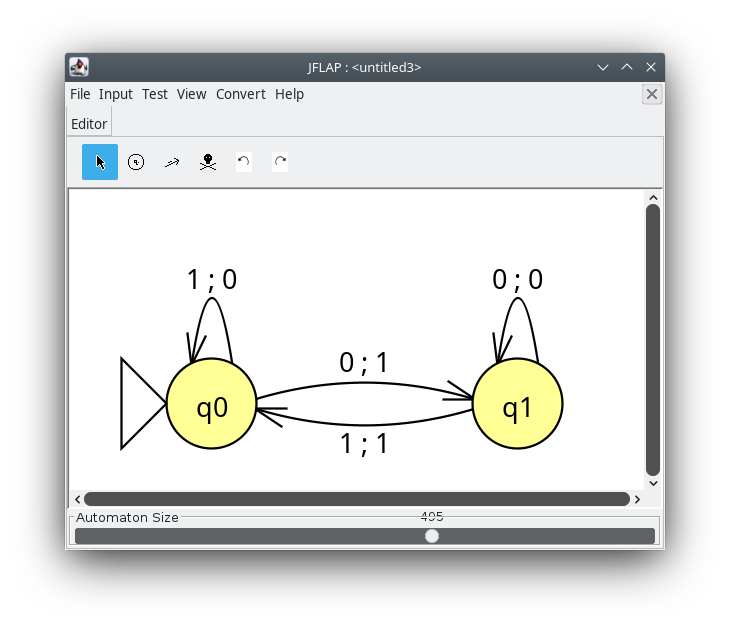
\includegraphics[scale=0.34]{Prácticas/Mealy - Decodificador}
	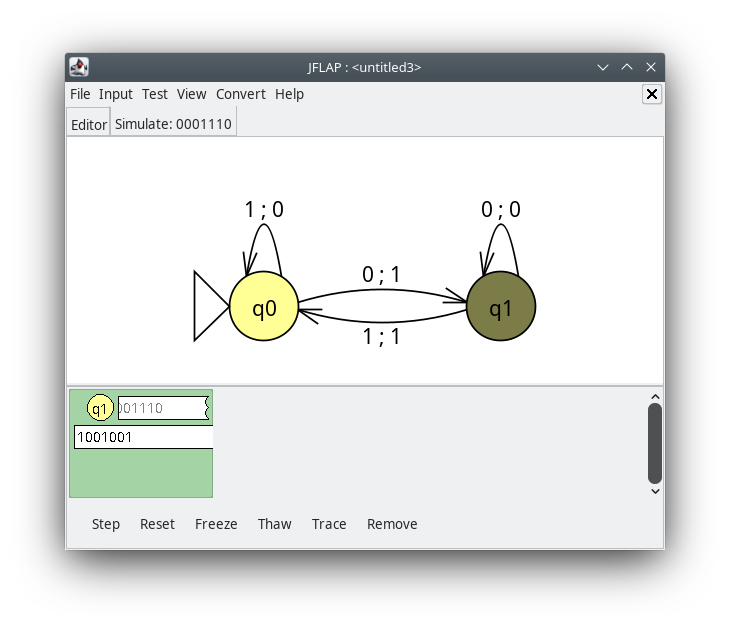
\includegraphics[scale=0.34]{Prácticas/Mealy - Decodificador ejecución}
\end{center}
\caption{Máquina de Mealy decodificadora.}
\end{figure}
